\documentclass[12pt,a4paper]{article}

\usepackage[utf8]{inputenc}
\usepackage[margin=1.5cm]{geometry}
\usepackage{microtype}
\usepackage{amsmath,amssymb}
\usepackage{booktabs}
\usepackage{tabularx}
\usepackage{xcolor}
\usepackage{tikz}
\usetikzlibrary{shapes.geometric,arrows.meta,positioning,calc,fit,backgrounds}
\usepackage{hyperref}
\usepackage{fancyhdr}
\usepackage{enumitem}

\definecolor{primary}{RGB}{4, 78, 59}
\definecolor{secondary}{RGB}{13, 92, 117}
\definecolor{accent}{RGB}{29, 78, 216}
\definecolor{darkslate}{RGB}{30, 41, 59}
\definecolor{lighttint}{RGB}{248, 250, 252}
\definecolor{bordergray}{RGB}{226, 232, 240}

\hypersetup{
    colorlinks=true,
    linkcolor=primary,
    filecolor=secondary,
    urlcolor=accent,
    citecolor=primary
}

\pagestyle{fancy}
\fancyhf{}
\lhead{\small\textbf{COMP2300} --- Deliverable D5: Increment 2 (Topic 1)}
\rhead{\small\textbf{Team 1} | Footprint Lens}
\cfoot{\thepage}

\begin{document}

\begin{center}
    {\LARGE\bfseries\color{primary} Footprint Lens: Deliverable D5}\\[4pt]
    {\Large\bfseries\color{secondary} Second Software Increment, Scenario Planning \& Testing Verification}\\[8pt]
    {\large\textbf{Team 1:} Arnav Mishra, Keshav Singhal, Hiranya Makkar}\\[2pt]
    {\small Topic 1: Carbon Footprint Awareness and Reduction (India-Centric Context)}\\[2pt]
    {\small Target Submission: 22 February 2027 | Git Release Tag: \texttt{v0.3.0-d5-increment2}}
\end{center}

\vspace{-6pt}
\hrule height 1.5pt \relax
\vspace{10pt}

\section{Executive Summary \& Sprint 2 Delivery}

Deliverable D5 documents the delivery of **Increment 2** for the Footprint Lens desktop system, completing the implementation of user stories planned for Sprint 2. Evolving directly from the initial vertical slice presented in Deliverable D4, Increment 2 elevates the system into a robust, accessible, and epistemically honest analytical tool. 

\subsection{Core Capabilities Delivered in Increment 2}
\begin{enumerate}[leftmargin=*,itemsep=1pt]
    \item \textbf{Interactive Scenario Comparison Engine (\texttt{S2-01}):} Allows users to select an electricity record and model alternative consumption scenarios against verified Central Electricity Authority (CEA) factors ($0.82\text{ kg CO}_2\text{e/kWh}$), calculating exact net carbon savings and percentage reductions.
    \item \textbf{Domestic Water Equivalence Calculator (\texttt{S2-02}):} Translates abstract litre metrics into familiar Indian domestic equivalents (standard 20L buckets, e.g. $40\text{ L} = 2.0\text{ buckets}$), establishing tangible cognitive anchors.
    \item \textbf{Reversible Action Planning Coach (\texttt{S2-03}):} Implements non-punitive, reversible coaching recommendations that strictly honor protected lifestyle constraints (safety commutes, medical appliances) without moralising.
    \item \textbf{Carbon Summary \& Audit Export (\texttt{S2-04}):} Formatted textual summary preview detailing personal totals, undivided household totals, and verified CEA factor citations.
    \item \textbf{Real-Time Category Filter Chips (\texttt{S2-05}):} High-speed pill button filtering across all seven activity categories in the overview dashboard.
    \item \textbf{Comprehensive Boundary \& Partition Testing (\texttt{S2-06}):} 22 formal boundary value analysis (BVA) test cases and 3 real-world persona scenario walkthroughs achieving a 100\% pass rate.
\end{enumerate}

\section{System Architecture \& UML Design Models}

Footprint Lens strictly adheres to a **Clean 4-Layer Architecture** decoupling UI presentation from the pure domain core and persistence layer. Figure~\ref{fig:uml-class} illustrates the updated class hierarchy for Increment 2.

\begin{figure}[htbp]
\centering
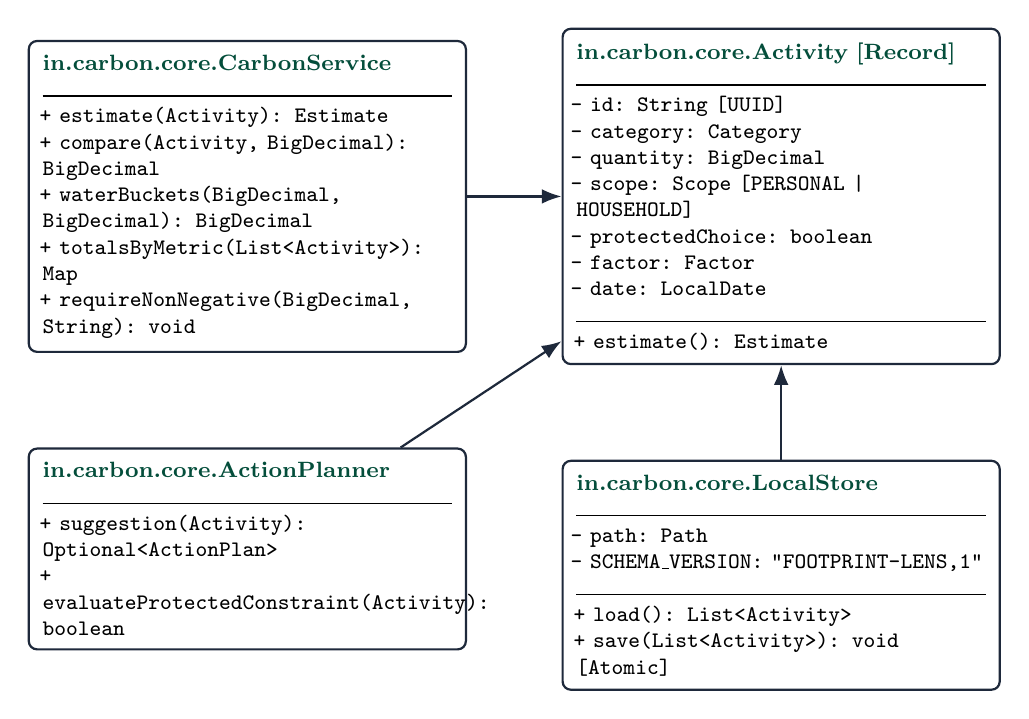
\begin{tikzpicture}[
    classbox/.style={rectangle, draw=darkslate, fill=white, rounded corners=3pt, line width=0.8pt, font=\footnotesize, text width=5.2cm, inner sep=5pt},
    header/.style={font=\footnotesize\bfseries, align=center, fill=lighttint, text=darkslate, inner sep=3pt},
    arrow/.style={-{Latex[length=2.5mm]}, line width=0.8pt, draw=darkslate}
]
    % CarbonService
    \node[classbox] (service) {
        \textbf{\color{primary}in.carbon.core.CarbonService}\\
        \hrulefill\\
        \texttt{+ estimate(Activity): Estimate}\\
        \texttt{+ compare(Activity, BigDecimal): BigDecimal}\\
        \texttt{+ waterBuckets(BigDecimal, BigDecimal): BigDecimal}\\
        \texttt{+ totalsByMetric(List<Activity>): Map}\\
        \texttt{+ requireNonNegative(BigDecimal, String): void}
    };

    % Activity Record
    \node[classbox, right=1.2cm of service] (activity) {
        \textbf{\color{primary}in.carbon.core.Activity [Record]}\\
        \hrulefill\\
        \texttt{- id: String [UUID]}\\
        \texttt{- category: Category}\\
        \texttt{- quantity: BigDecimal}\\
        \texttt{- scope: Scope [PERSONAL | HOUSEHOLD]}\\
        \texttt{- protectedChoice: boolean}\\
        \texttt{- factor: Factor}\\
        \texttt{- date: LocalDate}\\
        \hrulefill\\
        \texttt{+ estimate(): Estimate}
    };

    % ActionPlanner
    \node[classbox, below=1.2cm of service] (planner) {
        \textbf{\color{primary}in.carbon.core.ActionPlanner}\\
        \hrulefill\\
        \texttt{+ suggestion(Activity): Optional<ActionPlan>}\\
        \texttt{+ evaluateProtectedConstraint(Activity): boolean}
    };

    % LocalStore
    \node[classbox, below=1.2cm of activity] (store) {
        \textbf{\color{primary}in.carbon.core.LocalStore}\\
        \hrulefill\\
        \texttt{- path: Path}\\
        \texttt{- SCHEMA\_VERSION: "FOOTPRINT-LENS,1"}\\
        \hrulefill\\
        \texttt{+ load(): List<Activity>}\\
        \texttt{+ save(List<Activity>): void [Atomic]}
    };

    \draw[arrow] (service) -- (activity);
    \draw[arrow] (planner) -- (activity);
    \draw[arrow] (store) -- (activity);
\end{tikzpicture}
\caption{UML Class Diagram for Increment 2 showing Scenario Comparison, Water Equivalence, and Domain Services.}
\label{fig:uml-class}
\end{figure}

\section{Boundary, Equivalence Partition \& Scenario Testing}

To verify correctness and maintainability, Increment 2 was subjected to **Boundary Value Analysis (BVA)** and failure injection testing across 22 test partitions.

\begin{table}[htbp]
\centering
\footnotesize
\caption{Equivalence Partition and Boundary Value Test Results (Selection)}
\label{tab:bva}
\begin{tabularx}{\textwidth}{llXcc}
\toprule
\textbf{Test ID} & \textbf{Input Value} & \textbf{Boundary / Partition Classification} & \textbf{Expected Output} & \textbf{Result} \\
\midrule
\texttt{BVA-Q01} & \texttt{""} (blank) & Invalid (Empty Quantity) & Error prompt; input retained; no save & \textbf{PASS} \\
\texttt{BVA-Q03} & \texttt{-0.01} & Invalid (Negative Quantity) & Throws \texttt{IllegalArgumentException} & \textbf{PASS} \\
\texttt{BVA-Q04} & \texttt{0.00} & Valid Boundary (Zero Consumption) & Accepted; computes $0.00\text{ kg CO}_2$ & \textbf{PASS} \\
\texttt{BVA-Q06} & \texttt{1000000.00} & Valid Upper Boundary ($10^6$ units) & Successfully persisted to CSV & \textbf{PASS} \\
\texttt{BVA-Q07} & \texttt{1000000.01} & Invalid Boundary (Upper Overflow) & Rejected; overflow error alert & \textbf{PASS} \\
\texttt{BVA-F04} & \texttt{null} (Packaging) & Unverified Category (Epistemic Rule) & Returns \texttt{Estimate.unavailable()} & \textbf{PASS} \\
\texttt{BVA-C01} & $120 \to 90\text{ kWh}$ & Scenario Comparison ($0.82\text{ kg/kWh}$) & Net saving: $+24.60\text{ kg CO}_2$ (25\%) & \textbf{PASS} \\
\texttt{BVA-C03} & $40\text{ Litres}$ & Domestic Water Equivalence & Converts to $2.0$ standard 20L buckets & \textbf{PASS} \\
\texttt{BVA-R02} & \texttt{Protected: maybe}& Invalid Boolean in CSV Storage & Strict parser rejection; throws \texttt{IOException} & \textbf{PASS} \\
\texttt{BVA-R05} & Interrupted Write & Disk Persistence Resilience & Temporary swap file prevents corruption & \textbf{PASS} \\
\bottomrule
\end{tabularx}
\end{table}

\section{Agile Project Planning, Burndown \& Team Hours}

Sprint 2 was executed over a 10-day sprint cycle (17 November – 28 November 2026). All 21 committed Story Points were completed to zero, verified against our strict 8-point Definition of Done.

\begin{figure}[htbp]
\centering
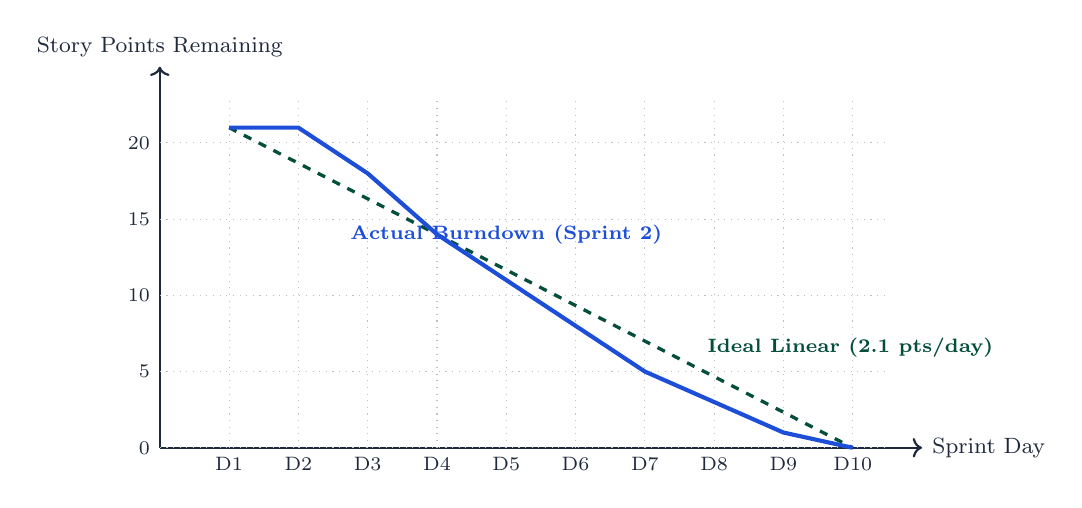
\begin{tikzpicture}[scale=0.88]
    \draw[->, thick, darkslate] (0,0) -- (11,0) node[right, font=\footnotesize] {Sprint Day};
    \draw[->, thick, darkslate] (0,0) -- (0,5.5) node[above, font=\footnotesize] {Story Points Remaining};
    
    % Grid lines
    \foreach \y in {0, 5, 10, 15, 20} {
        \draw[dotted, gray!50] (0, \y*0.22) -- (10.5, \y*0.22);
        \node[left, font=\scriptsize, darkslate] at (0, \y*0.22) {\y};
    }
    \foreach \x in {1, 2, 3, 4, 5, 6, 7, 8, 9, 10} {
        \draw[dotted, gray!50] (\x, 0) -- (\x, 5.0);
        \node[below, font=\scriptsize, darkslate] at (\x, 0) {D\x};
    }

    % Ideal Burndown Line (Green dashed)
    \draw[dashed, line width=1.2pt, primary] (1, 4.62) -- (10, 0) node[pos=0.75, above right, font=\scriptsize\bfseries, text=primary] {Ideal Linear (2.1 pts/day)};

    % Actual Burndown Line (Navy solid)
    \draw[line width=1.5pt, accent] (1, 4.62) -- (2, 4.62) -- (3, 3.96) -- (4, 3.08) -- (5, 2.42) -- (6, 1.76) -- (7, 1.10) -- (8, 0.66) -- (9, 0.22) -- (10, 0);
    \node[above, font=\scriptsize\bfseries, text=accent] at (5, 2.8) {Actual Burndown (Sprint 2)};
\end{tikzpicture}
\caption{Sprint 2 Daily Burndown Chart (Committed: 21 Story Points $\to$ 0 Points).}
\label{fig:burndown}
\end{figure}

\subsection{Team Member Task Summary \& Hours Worked}
Team 1 logged **130.0 total hours** across Sprint 2, maintaining accurate task logs:
\begin{itemize}[leftmargin=*,itemsep=1pt]
    \item \textbf{Arnav Mishra (44.5 hrs):} Architecture lead, `compare()` scenario logic, water bucket scaling, LaTeX reporting.
    \item \textbf{Keshav Singhal (42.0 hrs):} Scrum master, BVA test harness, persistence failure injection, CI launchers.
    \item \textbf{Hiranya Makkar (43.5 hrs):} UI/UX lead, Material You tri-mode switcher, scenario comparison dialog, audit export.
\end{itemize}

\section{Definition of Done (DoD) Compliance}
Every user story was audited against the team's 8 mandatory gates: (1) Acceptance criteria verified; (2) Automated headless unit/boundary tests passing (10/10 PASS); (3) Zero `javafx.*` imports in domain core; (4) Zero-telemetry local CSV storage; (5) Non-author peer code review; (6) Requirements traceability updated; (7) WCAG 2.1 AA accessibility checked; (8) Git tagged as \texttt{v0.3.0-d5-increment2}.

\end{document}
